\documentclass{fizraport}
\authorA{Krzysztof Stasiowski}
\authorB{Joanna Binek}
\team{2}{2a}{1}

\topic{Opracowanie danych pomiarowych}{0}
\carryOutDate{03.10.2018 r.}
\ftHandInDate{10.10.2018 r.}
\begin{document}

\maketitle

\section{Cel ćwiczenia}
Zaznajomienie się z typowymi metodami opracowania danych pomiarowych
przy wykorzystaniu wyników pomiarów dla wahadła prostego.

\section{Wstęp}
Wahadło proste jest, jak wskazuje jego nazwa, układem mechanicznym charakteryzującym się prostotą tak  eksperymentu  jak  i  opisu  teoretycznego.
Dlatego nadaje  się dobrze  na ćwiczenie  wprowadzające (zerowe),   mające   na   celu   poznanie   podstawowych   metod   opracowania danych   pomiarowych.
Interpretacja  wyników  opiera  się na  równaniu  określającym  okres  drgań $T$ jako  funkcję długości wahadła $l$ oraz przyspieszenia ziemskiego $g$, 
%
\[ T = 2\pi \sqrt{\frac{l}{g}} \]
%
Wzór ten jest słuszny, jeżeli wychylenie ciężarka z położenia równowagi jest małe.  
Przekształcając powyższy wzór możemy wyznaczyć wartość przyspieszenia ziemskiego:
%
\[ g = \frac{4\pi^2l}{T^2} \]

\section{Opis Doświadczenia}
\begin{wrapfigure}[19]{r}{0.34\textwidth}
 \centering
 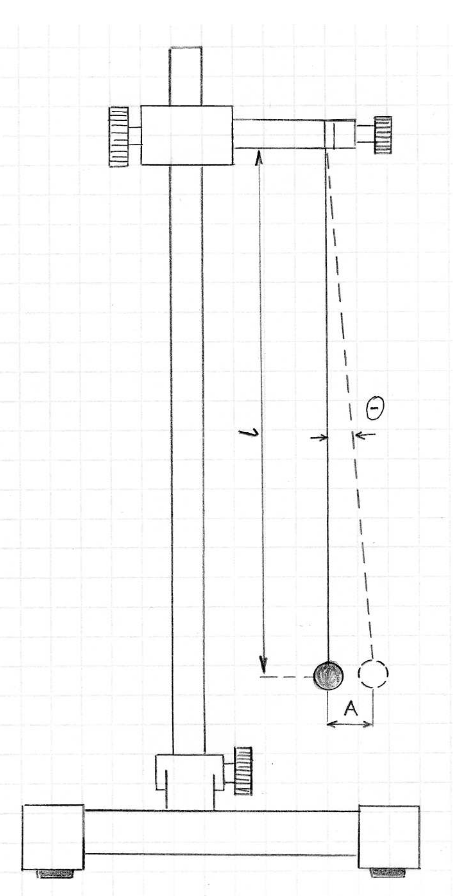
\includegraphics[width=0.27\textwidth,keepaspectratio=true]{wahadlo1.png}
 % wahadlo1.png: 474x896 px, 72dpi, 16.72x31.60 cm, bb=0 0 474 896
 \caption{Wahadło proste}
 \label{fig:w1}
\end{wrapfigure}

Zostały wykonane dwa rodzaje badań. Do obu zostało wykorzystane wahadło przedstawione na \figurename{\ref{fig:w1}}.

Składa się ono z~cylindrycznego mosiężnego odważnika zawieszonego na cienkiej lince. Linka została powieszona na wolnostojącym statywie - umożliwiającym regulację długości linki.
Pomiary były dokonywane za pomocą stopera o~dokładności~0.01s. Do niepewności pomiaru stopera należy dodać czas reakcji osoby wykonującej pomiary, który został ustalony na 0.1s.

Długość wahadła została zmierzona za pomocą linijki o~podziałce~1mm, niestety dokładność wyznaczenia długości jest mniejsza z~powodu konieczności oszacowanie środka masy cylindra i~została określona~na~5mm.


\subsection{Pomiary przy stałej długości linki}
Pierwszymi wykonanymi pomiarami była seria pomiarów okresu~($T$) przy stałej długości linki,którą zmierzyliśmy i~otrzymaliśmy wynik 37,5~cm. 

Wychyliliśmy wahadło o~niewielki kąt z~położenia równowagi i~puściliśmy. Następnie zmierzyliśmy przy pomocy stopera 20~pełnych okresów wahadła. Czynności te~powtórzyliśmy 15 razy i~uzyskaliśmy wyniki podane w~\tablename{\ref{T:equipos}}. 

\begin{table}[!ht]
\caption{Pomiar okresu drgań przy ustalonej długości wahadła}
\bigskip%\medskip%\smallskip % dobierz co będzie dobre
długość wahadła ~$l = 37,5 $cm \\ 
niepewność pomiaru ~$u(l) = 5$mm
\label{T:equipos}
\begin{center}
\begin{tabular}{| c | c | c | c | c |}
\hline
\textbf{Lp.} & \textbf{ liczba }      & \textbf{czas ~$t$ dla }           & \textbf{okres}   \\
             & \textbf{okresów ~$k$ } & \textbf{$k$ okresów $[\text{s}]$} & \textbf{$T = \frac{t}{k} [\text{s}]$}   \\
\hline

 1 & 20 & 23,41& 1,17\\ \hline
 2 & 20 & 24,09& 1,20\\ \hline
 3 & 20 & 24,28& 1,21\\ \hline
 4 & 20 & 24,44& 1,22\\ \hline
 5 & 20 & 24,53& 1,23\\ \hline
 6 & 20 & 24,56& 1,23\\ \hline
 7 & 20 & 24,78& 1,24\\ \hline
 8 & 20 & 24,87& 1,24\\ \hline
 9 & 20 & 24,87& 1,24\\ \hline
10 & 20 & 24,97& 1,25\\ \hline
11 & 20 & 25,03& 1,25\\ \hline
12 & 20 & 24,78& 1,24\\ \hline
13 & 20 & 25,07& 1,25\\ \hline
14 & 20 & 25,31& 1,27\\ \hline
15 & 20 & 25,75& 1,29\\ \hline
\end{tabular}
\end{center}
\end{table}

\subsection{Pomiary przy różnej długości linki}
Drugimi wykonanymi pomiarami była seria pomiarów okresu, przy~zmieniającej się długości linki~($l$). 

Ponownie zmierzyliśmy długość wahadła,następnie wychyliliśmy wahadło o~niewielki kąt z~położenia równowagi i~puściliśmy .  Zmierzyliśmy przy pomocy stopera 20 pełnych okresów wahadła, a~następnie zmieniliśmy długość wahadła. Czynności te~powtórzyliśmy 9 razy i~uzyskaliśmy wyniki podane~w~\tablename{\ref{T:varpos}}.


\begin{table}[!h]
\caption{Pomiar zależności okresu drgań od długości wahadła}
\label{T:varpos}
\begin{center}
\begin{tabular}{| c | c | c | c | c | c |}
\hline
\textbf{Lp.} & $l[\text{mm}]$
& $k$ & $t [\text{s}]$ & $T_i [\text{s}]$ & $T_i^2 [\text{s}^2]$  \\
\hline
1 & 375 & 20 & 24,97 & 1,25 & 1,56\\ \hline
2 & 135 & 20 & 14,81 & 0,74 & 0,55\\ \hline
3 & 215 & 20 & 18,72 & 0,94 & 0,88\\ \hline
4 & 250 & 20 & 20,56 & 1,02 & 1,06\\ \hline
5 & 285 & 20 & 21,60 & 1,08 & 1,17\\ \hline
6 & 320 & 20 & 22,82 & 1,14 & 1,30\\ \hline
7 & 350 & 20 & 23,53 & 1,18 & 1,38\\ \hline
8 & 75  & 20 & 10,91 & 0,55 & 0,30\\ \hline
9 & 120 & 20 & 13,90 & 0,70 & 0,48\\ \hline
10& 160 & 20 & 15,82 & 0,79 & 0,63\\ \hline

\end{tabular}
\end{center}
\end{table}
\begin{wrapfigure}[20]{r}{0.5\textwidth}
 \centering
  \caption{Wykres zależności okresu od długości wahadła $T(l)$}
 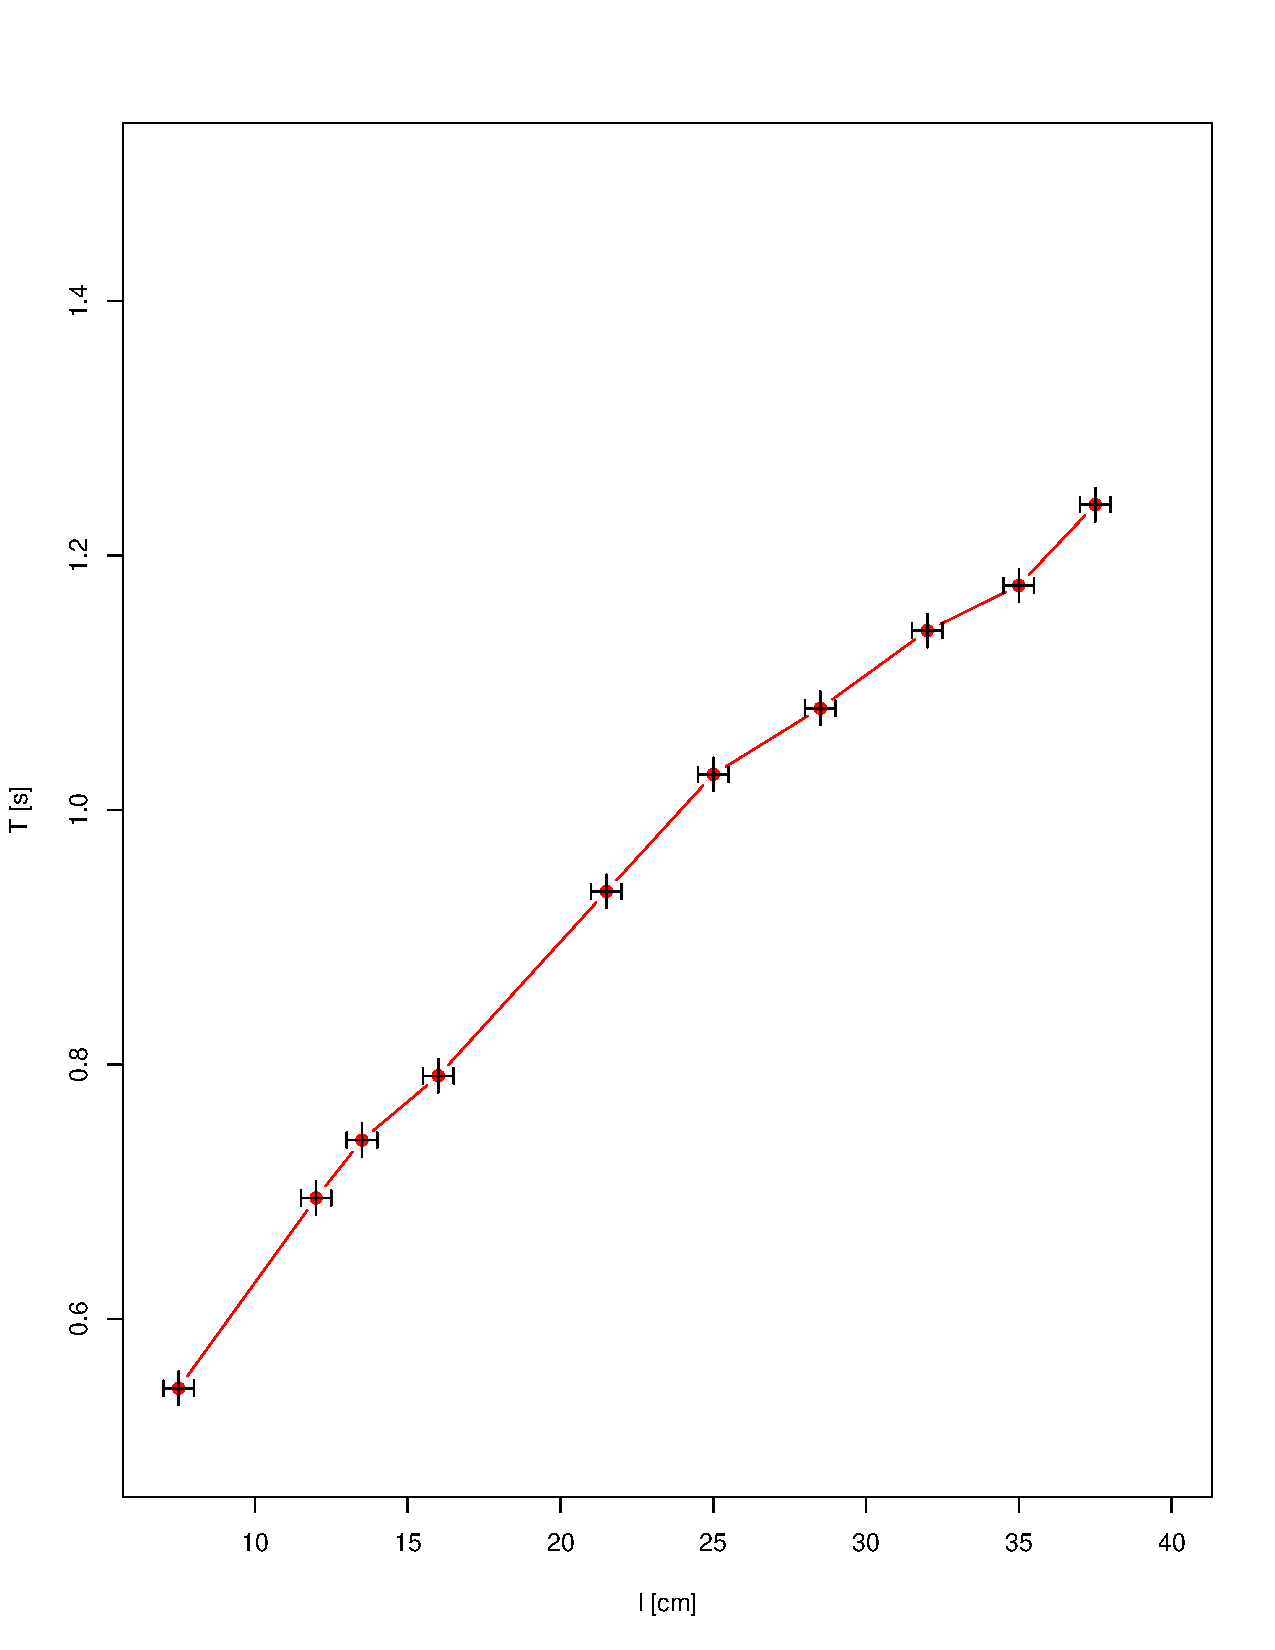
\includegraphics[width=0.5\textwidth,keepaspectratio=true]{WykresTodl.pdf}
 \label{fig:w2}
\end{wrapfigure}

\pagebreak
\section{Opracowanie wyników}
\subsection{Sprawdzenie czy wyniki pomiaru okresu nie zawierają błędów grubych}
Pomiędzy wynikami pomiaru okresu nie występują drastyczne różnice, wszystkie wartości oscylują wokół 25 sekund, W szczególności między najmniejszą ($23,42$ s), a największą ($25,75$ s) zmierzoną wartością okresu nie występuje duża różnica. Można zatem stwierdzić że wyniki pomiaru okresu nie są obarczone błędami grubymi.

\subsection{Obliczanie niepewności pomiaru okresu ($T$)}
Do obliczenia niepweności pomiaru okresu należy zastosować ocenę niepewności Typu~A.
Rozpoczęliśmy od policzenia średnjej arytmetycznej $T$ zgodnie ze wzorem.
\[ \bar{T} = \frac{1}{n}\sum{T_i} = 1.24\text{s}\]
Następnie wykorzystaliśmy ją do obliczenia odchylenia standardowego - przy pomocy odpowiedniego estymatora.
\[s_x=\sqrt{\frac{\sum{(x_i-\bar{x})^2}}{14}}=0.028s\]
i przekształciliśmy je do odchylenia standardowego średniej.
\[u(T)=s_{\bar{T}}=\frac{s_T}{\sqrt{15}}=0.0072s\]
\subsection{Obliczanie niepewności pomiaru długośći wachadła ($l$)}
Do obliczenia niepewności pomiaru długości wahadła należy zastosować ocenę niepewności Typu~B.
Pierwszym zastosowanym przyliżeniem jest skala podziału użytego przyrządu - w tym przypadku linijki z podziałką 1 mm. $u(l) \approx 1\text{mm}$ Ale niestety z powodu trudnośi wyznaczenia środka masy walca, należy tą wartość skorygować w górę do:
\[ u(l) \approx 5\text{mm}\]
\pagebreak
\subsection{Obliczenie przyspieszenia ziemskiego}
Przy pomocy uzyskanych wartości możemy wyliczyć przyspieszenie ziemskie.
Do tego celu wykorzystamy następujący wzór:
\[ g = \frac{4\pi^2l}{T^2} \approx \frac{{4 \cdot {3.14}^2 (375)}}{{1.24}^2} \approx 9630 \left[\frac{\text{mm}}{\text{s}^2}\right] = 9.63 \left[\frac{\text{m}}{\text{s}^2}\right]\]
\subsection{Obliczanie niepewności złożonej i rozszerzonej przyspieszenia ziemskiego}
Do obliczenia niepewności złożonej $u_c(g)$ wykorzystamy prawo przenoszenia niepewności.
Dla naszego równania ma ono formę:
\[\frac{u_c(g)}{g} = \sqrt{ \left[\frac{l}{g}\frac{\partial g}{\partial l}\frac{u(l)}{l}\right]^2+ \left[\frac{T}{g}\frac{\partial g}{\partial T}\frac{u(T)}{T}\right]^2 }
\]
\[\frac{l}{g}\frac{\partial g}{\partial l} = \frac{l}{\frac{4\pi^2 l}{T^2}}\cdot\frac{4\pi^2}{T^2} = \frac{l}{l}=1\]
\[\frac{T}{g}\frac{\partial g}{\partial T} = \frac{T}{\frac{4\pi^2 l}{T^2}}\cdot-2(4\pi^2l)T^{-3}=-2\]
\[\frac{u_c(g)}{g} = \sqrt{ \left[\frac{u(l)}{l}\right]^2+ \left[-2\frac{u(T)}{T}\right]^2 }\]
\[\frac{u_c(g)}{g} = \sqrt{ \left[\frac{5}{375}\right]^2+ 4\left[\frac{0.0072}{1.24}\right]^2 } = 0.018\]
Co pozwala nam na wyliczenie niepweności złożonej:
\[u_c(g) = 0.17 \left[\frac{m}{s^2}\right] \]
oraz niepewności rozszerzonej:
\[U(g) =k u_c(g) =2 \cdot 0.17 = 0.34\left[\frac{m}{s^2}\right] \]
Wyliczona przez nas wartość $g=9.63 \frac{m}{s^2} $ jest zgodna w granicach niepewnośći rozszerzonej z wartością tabelaryczną ($ g_t = 9.811 \frac{m}{s^2}$).
\pagebreak
\subsection{Wykonanie wykresu zależności $T^2$ w funkcji $l$}
W celu wykonania zlinearyzowanego wykresu  $T^2(l)$ posłużyliśmy się poprzednio zebranymi pomiarami długości linki, a wartości odpowiadających im okresów obliczyliśmy z następującego wzoru podniesionego do kwadratu:
%
\[ T = 2\pi \sqrt{\frac{l}{g}} \]
%
Zależności między wyliczonymi wartościami przedstawia wykres \figurename{\ref{fig:w3}}
\begin{figure}[htbp]
 \centering
  \caption{Zlinearyzowany wykres zależności wartości okresu podniesionej do kwadratu od długości wahadła $T^2(l)$}
 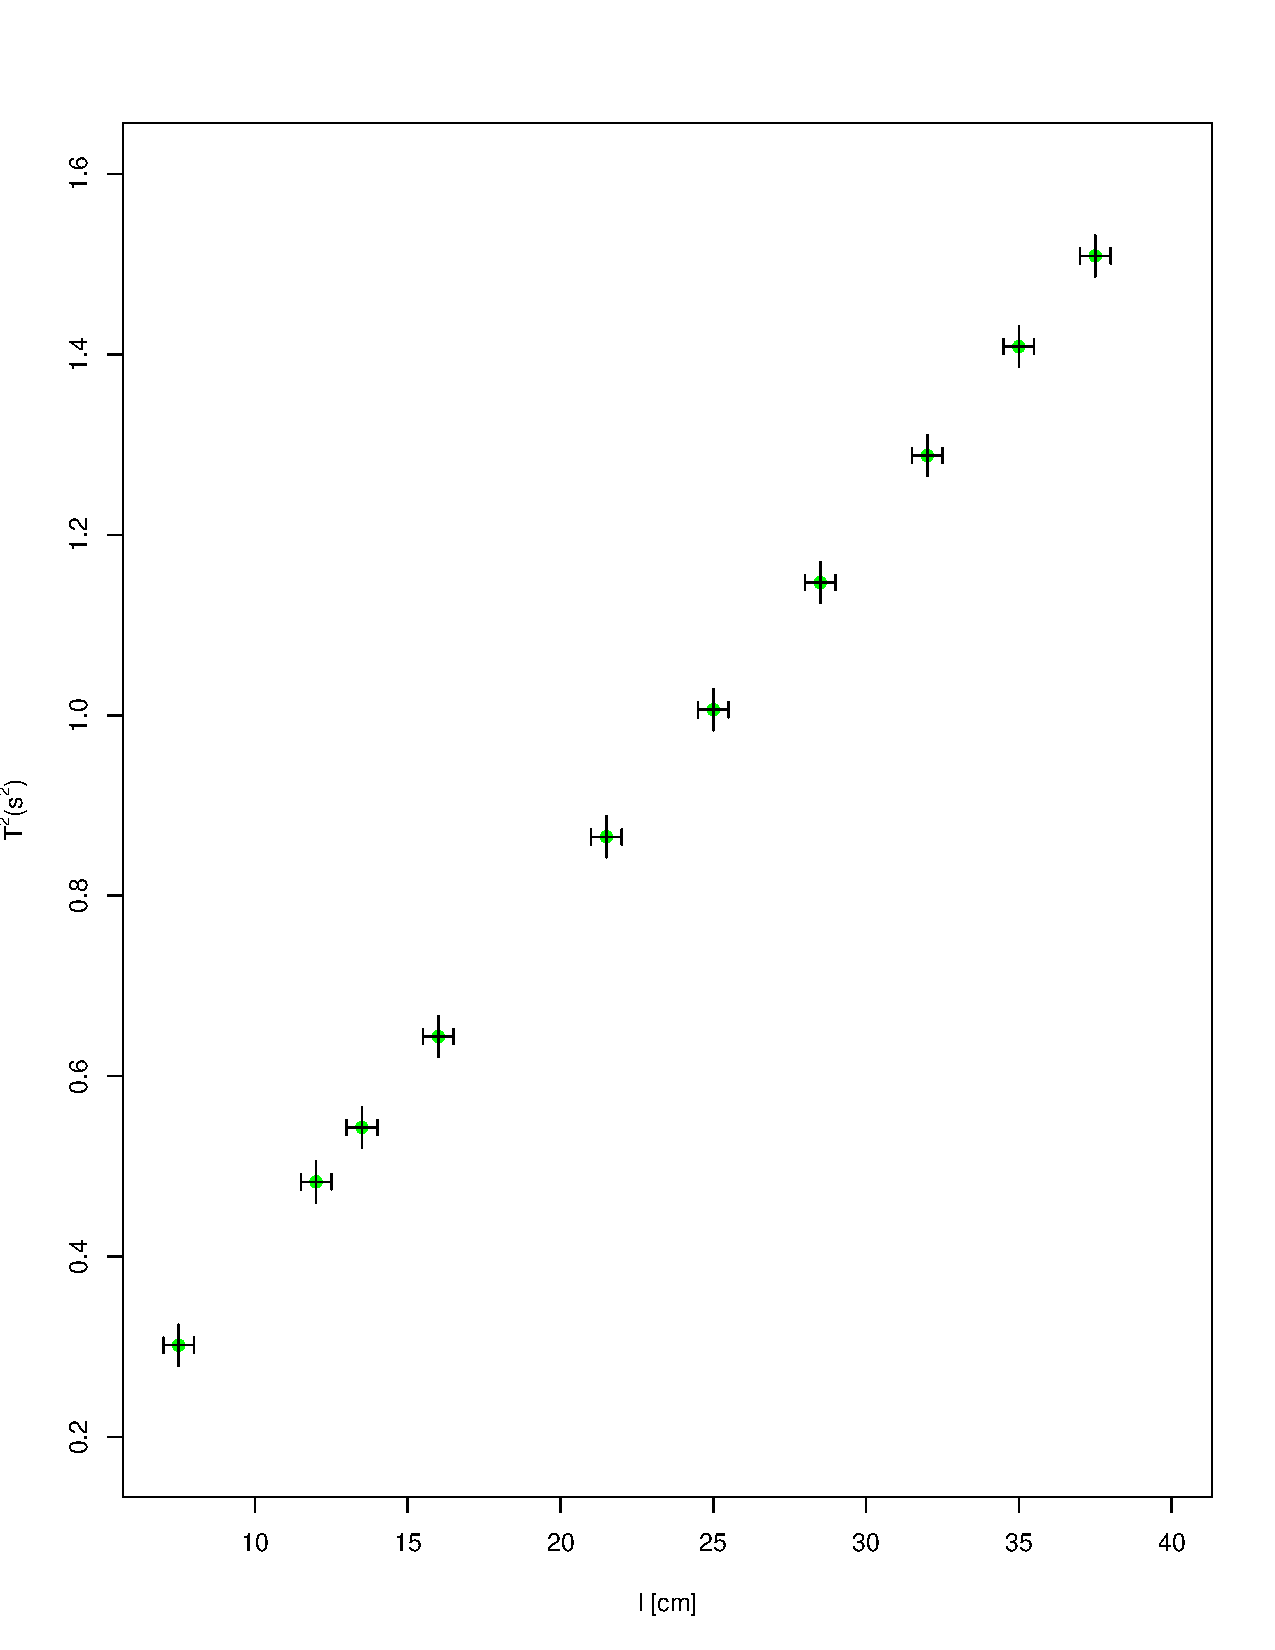
\includegraphics[width=0.8\textwidth,keepaspectratio=true]{wykres2.pdf}
 \label{fig:w3}
\end{figure}
\pagebreak
\subsection{Wyliczenie przyspieszenia ziemskiego na podstawie wykresu}
W pierwszej kolejności do naszych punktów doświadczalnych dobraliśmy prostą typu y = ax, czyli przechodzącą przez początek
układu współrzędnych. Skorzystaliśmy w tym celu z metody najmniejszych kwadratów.
%Za pomocą wykresu \figurename{\ref{fig:w3}} obliczyliśmy  wartość $g$.
\[ a = \frac{\sum{l_i \cdot T_i^2}}{\sum{l_i^2}}=4.06\]
W wyniku czego otrzymaliśmy prostą przedstawioną na wykresie~ \figurename{\ref{fig:w4}}
%TUTAJ
\begin{figure}[htbp]
 \centering
  \caption{Wykres prostej typu $y = ax$ dopasowanej do punktów doświadczalnych}
 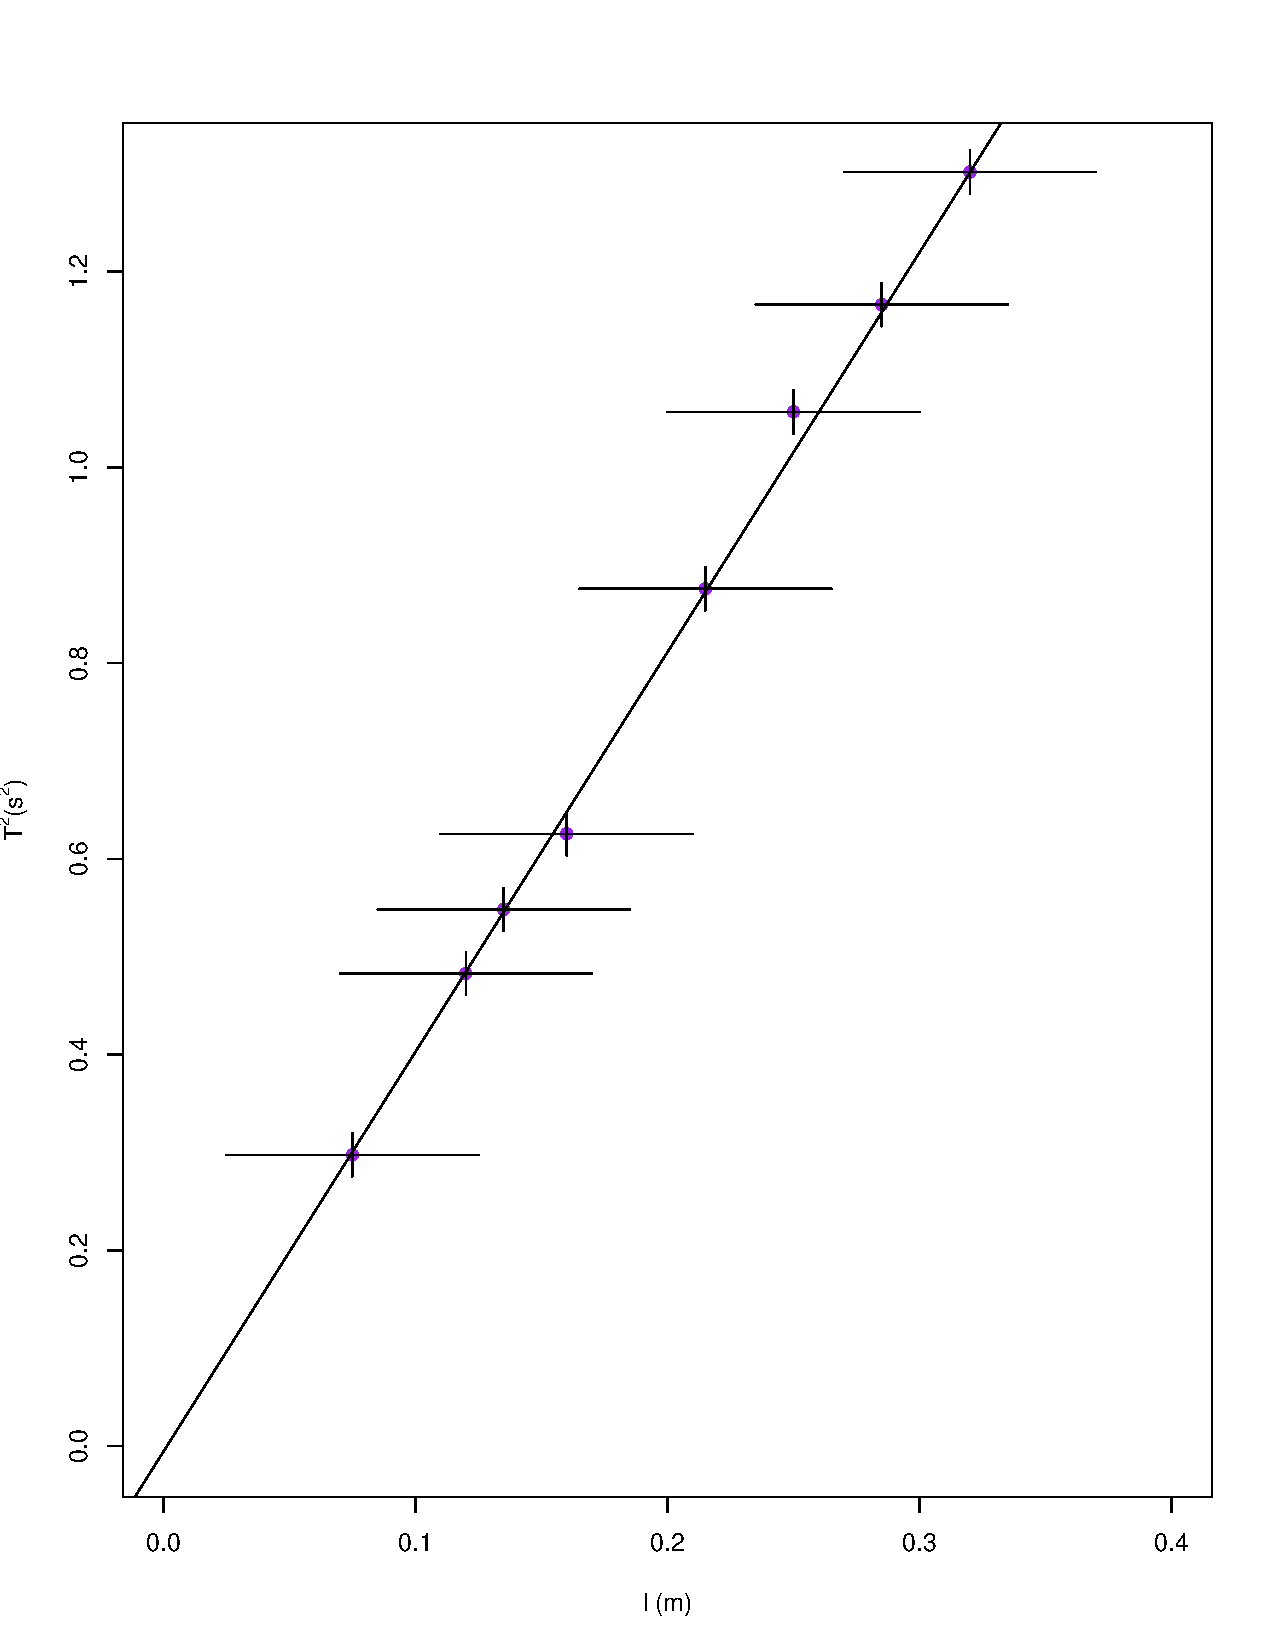
\includegraphics[width=0.5\textwidth,keepaspectratio=true]{wykres3.pdf}
 \label{fig:w4}
\end{figure}
%
\\
Następnie przy pomocy $a$~wyznaczyliśmy~wartość~$g$.
\[T^2=a \cdot l\]
\[g=\frac{4\pi^2l}{T^2}=\frac{4\pi^2l}{a\cdot l}=\frac{4\pi^2}{a}=9.71\]
Po wyliczeniu wartości $a$ i $g$ przeszliśmy do wyliczenia niepewności $u(a)$:
\[u(a)=\sqrt{\frac{\sum{[T^2_i-al_i]^2}}{9\sum{l_i^2}}}=0.03\]
 następnie wykorzystaliśmy ją do obliczenia $u(g)$ i $U(g)$:
\[u(g) = \left| \frac{\partial g}{\partial a}u(a)\right|=\left| \frac{-4\pi^2}{a^2}u(a)\right|=0.07\]
\[U(g)=2u(g)=0.14\]
Wyznaczona wartość $g$ nie pokrywa się z wartością tabelaryczną $g_t$ w granicch niepewności standardowej $|g-g_t|>u(g)$. Natomiast znajduje się w granicach niepewności rozszerzonej $|g-g_t|<U(g)$.

\section{Podsumowanie}
Wyliczone za pomocą obu prezentowanych metod wartości $g$ (przyspieszenia ziemskiego) zgadzają się z wartościami tabelarycznymi dla tego parametru. Różnica między wynikami obliczeń dokonanych obiemia metodami nie jest znacząca, co jest spowodowane stosunkowo niewielką liczbą pomiarów i brakiem błędów grubych.
Zarówno pierwsza jak i druga metoda dobrze przybliżają faktczną wartość przyspieszenia ziemskiego $g$.
\end{document}


























